\documentclass{beamer}


\usepackage[T2A]{fontenc}
\usepackage[utf8]{inputenc}
\usepackage[english,russian]{babel}
\pdfmapfile{+sansmathaccent.map}


\mode<presentation>
{
	\usetheme{Warsaw} % or try Darmstadt, Madrid, Warsaw, Rochester, CambridgeUS, ...
	\usecolortheme{seahorse} % or try seahorse, beaver, crane, wolverine, ...
	\usefonttheme{serif}  % or try serif, structurebold, ...
	\setbeamertemplate{navigation symbols}{}
	\setbeamertemplate{caption}[numbered]
} 


%%%%%%%%%%%%%%%%%%%%%%%%%%%%
% itemize settings


%%%%%%%%%%%%%%%%%%%%%%%%%%%%
% itemize settings

\definecolor{myhotpink}{RGB}{255, 80, 200}
\definecolor{mywarmpink}{RGB}{255, 60, 160}
\definecolor{mylightpink}{RGB}{255, 80, 200}
\definecolor{mypink}{RGB}{255, 30, 80}
\definecolor{mydarkpink}{RGB}{155, 25, 60}

\definecolor{mypaleblue}{RGB}{240, 240, 255}
\definecolor{mylightblue}{RGB}{120, 150, 255}
\definecolor{myblue}{RGB}{90, 90, 255}
\definecolor{mygblue}{RGB}{70, 110, 240}
\definecolor{mycourseblue}{RGB}{120, 140, 255}
\definecolor{mycourselightblue}{RGB}{245, 250, 255}
\definecolor{mydarkblue}{RGB}{0, 0, 180}
\definecolor{myblackblue}{RGB}{40, 40, 120}

\definecolor{mygreen}{RGB}{0, 200, 0}
\definecolor{mygreen2}{RGB}{245, 255, 230}
\definecolor{mydarkgreen}{RGB}{0, 120, 0}
\definecolor{mydarkgreen}{RGB}{0, 120, 0}


\definecolor{mygray}{gray}{0.8}
\definecolor{mydarkgray}{RGB}{80, 80, 160}
\definecolor{mylightgray}{RGB}{160, 160, 160}

\definecolor{mydarkred}{RGB}{160, 30, 30}
\definecolor{mylightred}{RGB}{255, 150, 150}
\definecolor{myred}{RGB}{200, 110, 110}
\definecolor{myblackred}{RGB}{120, 40, 40}

\definecolor{mypink}{RGB}{255, 30, 80}
\definecolor{myhotpink}{RGB}{255, 80, 200}
\definecolor{mywarmpink}{RGB}{255, 60, 160}
\definecolor{mylightpink}{RGB}{255, 80, 200}
\definecolor{mydarkpink}{RGB}{155, 25, 60}
\definecolor{mywhitepink}{RGB}{255, 240, 240}

\definecolor{mydarkcolor}{RGB}{60, 25, 155}
\definecolor{mylightcolor}{RGB}{130, 180, 250}



\setbeamertemplate{itemize items}[default]

\setbeamertemplate{itemize item}{\color{myblackblue}$\blacksquare$}
\setbeamertemplate{itemize subitem}{\color{mygblue}$\blacktriangleright$}
\setbeamertemplate{itemize subsubitem}{\color{mygray}$\blacksquare$}

\setbeamercolor{palette quaternary}{fg=white,bg=mycourseblue}
\setbeamercolor{titlelike}{parent=palette quaternary}

\setbeamercolor{palette quaternary2}{fg=black,bg=mycourselightblue}
\setbeamercolor{frametitle}{parent=palette quaternary2}

\setbeamerfont{frametitle}{size=\Large,series=\scshape}
\setbeamerfont{framesubtitle}{size=\normalsize,series=\upshape}





%%%%%%%%%%%%%%%%%%%%%%%%%%%%
% block settings

\setbeamercolor{block title}{bg=red!30,fg=black}

\setbeamercolor*{block title example}{bg=mygreen!40!white,fg=black}

\setbeamercolor*{block body example}{fg= black, bg= mygreen2}


%%%%%%%%%%%%%%%%%%%%%%%%%%%%
% URL settings
\hypersetup{
	colorlinks=true,
	linkcolor=blue,
	filecolor=blue,      
	urlcolor=blue,
}

%%%%%%%%%%%%%%%%%%%%%%%%%%

\renewcommand{\familydefault}{\rmdefault}


\newcommand{\mycolor}[1] {
\setbeamercolor{normal text}{fg={#1}} % Recolors standard body text
\setbeamercolor{structure}{fg={#1}}   % Recolors bullets and structure items
\usebeamercolor[fg]{normal text}      % Applies the normal text color immediately
}


\usepackage{amsmath}
\usepackage{mathtools}

\usepackage{cancel}
\usepackage{centernot}

\usepackage{changepage}
\usepackage{subcaption}

\usepackage{qrcode}

\newcommand{\bo}[1] {\mathbf{#1}}
\newcommand{\R}{\mathbb{R}} 
\newcommand{\T}{^\top}     



\newcommand{\mydate}{Fall 2026}

\newcommand{\mygit}{\textcolor{blue}{\href{https://github.com/SergeiSa/Advanced-Control-2026}{github.com/SergeiSa/Advanced-Control-2026}}}

\newcommand{\myqr}{ \textcolor{black}{\qrcode[height=1.5in]{https://github.com/SergeiSa/Advanced-Control-2026}}
}




\newcommand{\bref}[2] {\textcolor{blue}{\href{#1}{#2}}}

%%%%%%%%%%%%%%%%%%%%%%%%%%%%
% code settings

\usepackage{listings}
\usepackage{color}
% \definecolor{mygreen}{rgb}{0,0.6,0}
% \definecolor{mygray}{rgb}{0.5,0.5,0.5}
\definecolor{mymauve}{rgb}{0.58,0,0.82}
\lstset{ 
	backgroundcolor=\color{white},   % choose the background color; you must add \usepackage{color} or \usepackage{xcolor}; should come as last argument
	basicstyle=\footnotesize,        % the size of the fonts that are used for the code
	breakatwhitespace=false,         % sets if automatic breaks should only happen at whitespace
	breaklines=true,                 % sets automatic line breaking
	captionpos=b,                    % sets the caption-position to bottom
	commentstyle=\color{mygreen},    % comment style
	deletekeywords={...},            % if you want to delete keywords from the given language
	escapeinside={\%*}{*)},          % if you want to add LaTeX within your code
	extendedchars=true,              % lets you use non-ASCII characters; for 8-bits encodings only, does not work with UTF-8
	firstnumber=0000,                % start line enumeration with line 0000
	frame=single,	                   % adds a frame around the code
	keepspaces=true,                 % keeps spaces in text, useful for keeping indentation of code (possibly needs columns=flexible)
	keywordstyle=\color{blue},       % keyword style
	language=Octave,                 % the language of the code
	morekeywords={*,...},            % if you want to add more keywords to the set
	numbers=left,                    % where to put the line-numbers; possible values are (none, left, right)
	numbersep=5pt,                   % how far the line-numbers are from the code
	numberstyle=\tiny\color{mygray}, % the style that is used for the line-numbers
	rulecolor=\color{black},         % if not set, the frame-color may be changed on line-breaks within not-black text (e.g. comments (green here))
	showspaces=false,                % show spaces everywhere adding particular underscores; it overrides 'showstringspaces'
	showstringspaces=false,          % underline spaces within strings only
	showtabs=false,                  % show tabs within strings adding particular underscores
	stepnumber=2,                    % the step between two line-numbers. If it's 1, each line will be numbered
	stringstyle=\color{mymauve},     % string literal style
	tabsize=2,	                   % sets default tabsize to 2 spaces
	title=\lstname                   % show the filename of files included with \lstinputlisting; also try caption instead of title
}


%%%%%%%%%%%%%%%%%%%%%%%%%%%%
% URL settings
\hypersetup{
	colorlinks=false,
	linkcolor=blue,
	filecolor=blue,      
	urlcolor=blue,
}

%%%%%%%%%%%%%%%%%%%%%%%%%%

%%%%%%%%%%%%%%%%%%%%%%%%%%%%
% tikz settings

\usepackage{tikz}
\tikzset{every picture/.style={line width=0.75pt}}


\newcommand{\myqrframe}{
	\begin{frame}
		\begin{center}
			\centerline{Слайды доступны на Github:}
			\bigskip
			\centerline{\mygit}
			\bigskip
			\myqr
		\end{center}
	\end{frame}
}


\subtitle{Современные методы управления роботами}
\author{Сергей Савин}
\date{2026}
\title{Collocation, Direct Shooting}



\begin{document}
	\maketitle
	
	\begin{frame}{Содержание}
		\begin{itemize}
			\item Напоминание: задача оптимизации траектории
			\item Параметризация функций: последовательность точек и сплайны
			\item Кубические сплайны Эрмита
			\item Функция стоимости и ограничения
			\item Коллокация: кодирование динамики в дискретных точках
			\item Прямое прицеливание и интегрирование Рунге--Кутты
			\item Пример: раскачивание перевёрнутого маятника
			\item Литература
		\end{itemize}
	\end{frame}
	
	
	
	
	\begin{frame}{Напоминание: Оптимизация траектории}
		\begin{flushleft}
			Оптимизация траектории --- это задача поиска
			\emph{допустимой траектории}, минимизирующей выбранную
			функцию стоимости.
			
			\vspace{0.5em}
			
			Например, мы можем сформулировать задачу как
			\[
			\begin{aligned}
				\min_{x(t),u(t),T}\quad
				&
				\Phi\bigl(x(T)\bigr)
				+
				\int_0^T L\bigl(x(t),u(t)\bigr)\,dt
				\\
				\text{s.t.}\quad
				&
				\dot{x}(t)=f\bigl(x(t),u(t)\bigr),
				\\
				&
				x(0)=x_A,
				\qquad
				x(T)=x_B.
			\end{aligned}
			\]
			
			\begin{itemize}
				\item $\Phi(x(T))$ --- это \textbf{терминальная стоимость}, которая
				штрафует конечное состояние.
				
				\item $L(x(t),u(t))$ --- это \textbf{стоимость движения}, которая
				штрафует состояние и управление вдоль траектории.
			\end{itemize}
			
			Конкретный выбор $\Phi$ и $L$ зависит от того, чего
			мы хотим достичь с помощью траектории.
		\end{flushleft}
	\end{frame}
	
	
	\begin{frame}{Сплайны}
		\begin{flushleft}
			\emph{Сплайн} --- это гладкая кусочно-полиномиальная функция.
			
			\vspace{0.5em}
			
			Для заданного набора узлов
			\[
			t_1 < t_2 < \cdots < t_N,
			\]
			сплайн определяется на каждом интервале $[t_i,t_{i+1}]$ как
			\[
			S_i(t)
			=
			a_i
			+b_i(t-t_i)
			+c_i(t-t_i)^2
			+\cdots
			+d_i(t-t_i)^K.
			\]
			
			\vspace{0.5em}
			
			Полиномы гладко соединяются в узлах. Например,
			\[
			S_i(t_i)=S_{i+1}(t_i),
			\]
			\[
			S_i'(t_i)=S_{i+1}'(t_i),
			\qquad
			S_i''(t_i)=S_{i+1}''(t_i),
			\quad \ldots
			\]
			
			Таким образом, сплайн может представлять гладкую функцию,
			используя лишь конечное число параметров.
		\end{flushleft}
	\end{frame}
	
	
	
	
	\begin{frame}{Параметризация функций: последовательность точек}
		\begin{flushleft}
			
			\begin{figure}
				\centering
				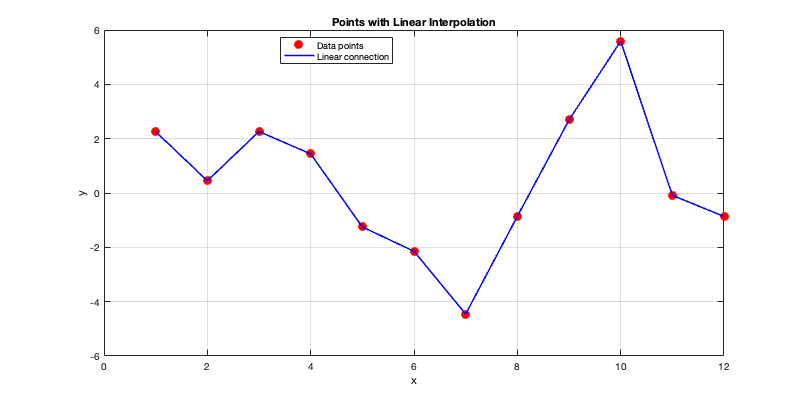
\includegraphics[width=1.1\linewidth]{illustration1}
				\caption{Последовательность точек}
				\label{fig:illustration1}
			\end{figure}
			
		\end{flushleft}
	\end{frame}
	
	
	
	
	\begin{frame}{Параметризация функций: сплайн}
		\begin{flushleft}
			
			\begin{figure}
				\centering
				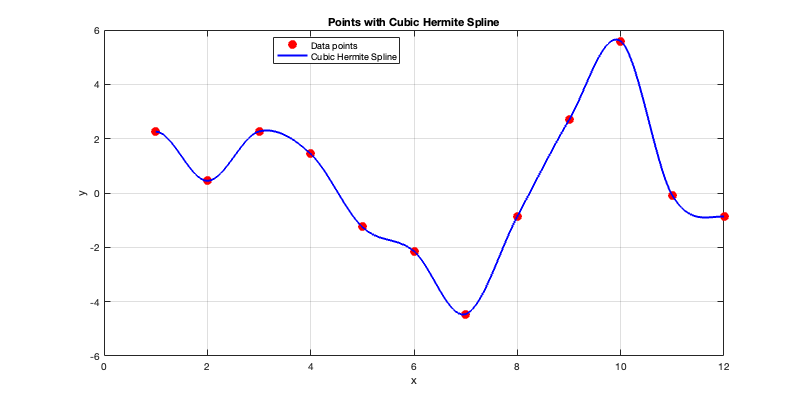
\includegraphics[width=1.1\linewidth]{illustration2}
				\caption{Кубический сплайн Эрмита}
				\label{fig:illustration1}
			\end{figure}
			
		\end{flushleft}
	\end{frame}
	
	
	
	\begin{frame}{Кубический сплайн Эрмита}
		\begin{flushleft}
			Кубический сплайн Эрмита строится из полиномов третьей степени
			между последовательными узлами.
			
			\vspace{0.5em}
			
			Для $t\in[t_i,t_{i+1}]$ определим нормированное время
			\[
			\tau
			=
			\frac{t-t_i}{t_{i+1}-t_i},
			\qquad
			\tau\in[0,1].
			\]
			
			Сплайн имеет вид
			\[
			S_i(t)
			=
			P_i h_{00}(\tau)
			+
			T_i h_{10}(\tau)
			+
			P_{i+1} h_{01}(\tau)
			+
			T_{i+1} h_{11}(\tau),
			\]
			где $P_i$ --- значение, а $(t_{i+1}-t_i)T_i$ --- производная
			в $i$-м узле. Базисные функции кубического сплайна Эрмита:
			\[
			\begin{aligned}
				h_{00}(\tau) &= 2\tau^3-3\tau^2+1, & h_{01}(\tau) &= -2\tau^3+3\tau^2, \\
				h_{10}(\tau) &= \tau^3-2\tau^2+\tau, & h_{11}(\tau) &= \tau^3-\tau^2.
			\end{aligned}
			\]
			
			
			Эти базисные функции обеспечивают заданные значения
			и производные на обоих концах.
		\end{flushleft}
	\end{frame}
	
	
	
	\begin{frame}{Сплайны в планировании траектории}
		\begin{flushleft}
			{\small
			
			В планировании траектории нам нужно заменить непрерывные
			функции $u(t)$ и $x(t)$ конечным набором параметров.
			
			\vspace{0.5em}
			
			Один из вариантов --- представить функции их значениями
			в конечном наборе точек:
			\[
			u(t)
			\quad\longrightarrow\quad
			\{u_1,u_2,\ldots,u_N\}.
			\]
			
			В качестве альтернативы мы можем параметризовать их с помощью сплайнов:
			\[
			u(t)=u(c,t),
			\]
			где $c$ содержит коэффициенты сплайна или значения в узлах.
			
			\vspace{0.3em}
			
			Сплайны обеспечивают гладкую аппроксимацию траектории
			и позволяют избежать разрывов.
			
			\vspace{0.3em}
			
			Однако гладкость не всегда желательна:
			\[
			\text{``нажать на газ''}
			\quad\longrightarrow\quad
			\text{``нажать на тормоз''}
			\]
			может естественно потребовать разрывного управляющего воздействия.
		}
		\end{flushleft}
	\end{frame}
	
	
	\begin{frame}{Функция стоимости}
		\begin{flushleft}
			
			{\small 
			Функция стоимости зависит от задачи, которую мы пытаемся
			решить. Однако несколько общих целей часто встречаются
			в планировании траектории.
			
			\vspace{0.5em}
			
			Для задачи перехода из $x_A$ в $x_B$ за $N$ шагов
			мы можем хотеть:
			
			\textbullet  достичь желаемого конечного состояния: $\|x_N-x_B\|^2$;
			
			\textbullet  \mbox{поддерживать близость последовательных состояний: $\sum\limits_{i=0}^{N-1}\|x_{i+1}-x_i\|^2$;}
			
			\textbullet  использовать малые управляющие воздействия: $\sum_{i=0}^{N-1}\|u_i\|^2$.
			
			\bigskip
			
			Эти цели можно объединить в единую стоимость:
			\[
			\min
			\quad
			w_1\|x_N-x_B\|^2
			+
			w_2\sum_{i=0}^{N-1}\|x_{i+1}-x_i\|^2
			+
			w_3\sum_{i=0}^{N-1}\|u_i\|^2.
			\]
			
			Веса $w_1,w_2,w_3$ определяют относительную
			важность различных целей.
		}
		\end{flushleft}
	\end{frame}
	
	
	\begin{frame}{Квадратичная стоимость общего вида}
		\begin{flushleft}
			Распространённый выбор функции стоимости --- квадратичная стоимость:
			\[
			\min
			\quad
			x_N^\top Q_N x_N
			+
			\sum_{i=0}^{N-1}
			\left(
			x_i^\top Q x_i
			+
			u_i^\top R u_i
			\right),
			\]
			где $Q_N\succeq 0,
			\quad
			Q\succeq 0,
			\quad
			R\succ 0$
			--- весовые матрицы.
			
			\vspace{0.5em}
			
			Если $u(t)$ или $x(t)$ параметризованы с помощью сплайна,
			мы можем вычислить сплайн в любой желаемой момент времени $t_i$. Точки вычисления не обязаны совпадать
			с узлами сплайна.
			
			\vspace{0.5em}
			
			Например, если $u(t)=a+bt$,
			то вычисление $J = \sum u_i^2$ в
			\[
			t_i\in\{0,0.5,1\}
			\]
			даёт
			\[
			J
			=
			a^2
			+
			(a+0.5b)^2
			+
			(a+b)^2.
			\]
		\end{flushleft}
	\end{frame}
	
	
	\begin{frame}{Ограничения}
		\begin{flushleft}
			Задачи планирования траектории часто включают ограничения,
			которые описывают, какие траектории физически или
			геометрически допустимы.
			
			\vspace{0.5em}
			
			Распространённые примеры включают:
			\begin{itemize}
				\item Ограничения по моменту:
				\[
				|u_i|\leq u_{\max}.
				\]
				
				\item Ограничения по шарнирам и скорости:
				\[
				x_{\min}\leq x_i\leq x_{\max}.
				\]
				
				\item Ограничения самопересечения.
				
				\item Избегание препятствий и столкновений.
				
				\item Ограничения контакта и захвата.
			\end{itemize}
			
			\vspace{0.5em}
			
			Мы также обычно накладываем начальные и конечные условия
			как ограничения:
			\[
			x_0=x_A,
			\qquad
			x_N=x_B.
			\]
		\end{flushleft}
	\end{frame}
	
	\begin{frame}{Коллокация}
		\begin{flushleft}
			Перед нами остаётся задача кодирования динамики системы:
			\[
			\dot{x}=f(x,u).
			\]
			
			\vspace{0.5em}
			
			\emph{Коллокация} обеспечивает выполнение динамики в конечном
			числе моментов времени, называемых \emph{точками коллокации}.
			
			\vspace{0.5em}
			
			Рассмотрим простой случай, когда $x(t)$ и $u(t)$
			представлены своими значениями
			\[
			x_0,x_1,\ldots,x_N,
			\qquad
			u_0,u_1,\ldots,u_{N-1}.
			\]
			
			Аппроксимируя производную с помощью конечной разности,
			\[
			\dot{x}(t_i)
			\approx
			\frac{x_{i+1}-x_i}{t_{i+1}-t_i},
			\]
			мы получаем ограничения коллокации
			\[
			\frac{x_{i+1}-x_i}{t_{i+1}-t_i}
			=
			f(x_i,u_i),
			\qquad
			i=0,\ldots,N-1.
			\]
		\end{flushleft}
	\end{frame}
	
	\begin{frame}{Коллокация: свойства}
		\begin{flushleft}
			Подход коллокации к обработке динамики имеет
			отличительные свойства:
			
			\vspace{0.5em}
			
			\begin{itemize}
				\item Динамика обеспечивается только в конечном числе
				точек коллокации.
				
				\vspace{0.5em}
				
				\item Переменные решения включают состояния
				\[
				x_0,x_1,\ldots,x_N
				\]
				и управления
				\[
				u_0,u_1,\ldots,u_{N-1}.
				\]
				
				\vspace{0.5em}
				
				\item В качестве альтернативы $x(t)$ и $u(t)$ могут быть представлены
				с помощью сплайнов или других параметризаций.
				
				\vspace{0.5em}
				
				\item Получающаяся задача оптимизации содержит
				явные ограничения, представляющие динамику системы.
			\end{itemize}
		\end{flushleft}
	\end{frame}
	
	\begin{frame}{Прямое прицеливание}
		\begin{flushleft}
			
			{\small 
				В отличие от коллокации, \emph{прямое прицеливание} кодирует
				динамику через схему численного интегрирования.
				
				\vspace{0.5em}
				
				Для заданного начального состояния $x_0$ и управляющих воздействий
				$u_0,u_1,\ldots$ состояния генерируются путём распространения
				динамики вперёд по времени.
				
				\vspace{0.5em}
				
				Например, используя метод Эйлера,
				\[
				x_{i+1}
				=
				x_i
				+
				f(x_i,u_i)
				(t_{i+1}-t_i).
				\]
				
				Начиная с $x_0$, это даёт
				\[
				x_1=x_1(u_0),
				\qquad
				x_2=x_2(u_0,u_1),
				\qquad\ldots
				\]
				
				Таким образом, состояния являются \emph{выражениями параметров
					управления}, а не независимыми переменными решения.
				
				\vspace{0.5em}
				
				При интегрировании методом Эйлера это алгебраически эквивалентно
				предыдущим дискретизированным ограничениям динамики. Различие становится важным при использовании более сложных
				схем интегрирования.
			}
		\end{flushleft}
	\end{frame}
	
	
	\begin{frame}{Интегрирование Рунге--Кутты}
		\begin{flushleft}
			Вместо метода Эйлера мы можем использовать схему
			интегрирования более высокого порядка, такую как метод Рунге--Кутты четвёртого порядка (RK4).
			
			\vspace{0.5em}
			
			Для шага по времени $h=t_{i+1}-t_i$ определим
			\[
			\begin{aligned}
				k_1 &= f(x_i,u_i),\\
				k_2 &= f\left(x_i+\frac{h}{2}k_1,u_i\right),\\
				k_3 &= f\left(x_i+\frac{h}{2}k_2,u_i\right),\\
				k_4 &= f\left(x_i+h k_3,u_i\right).
			\end{aligned}
			\]
			
			\vspace{0.5em}
			
			Затем состояние распространяется согласно
			\[
			x_{i+1}
			=
			x_i
			+
			\frac{h}{6}
			\left(
			k_1+2k_2+2k_3+k_4
			\right).
			\]
			
			Таким образом, при прямом прицеливании вся траектория
			получается путём повторного применения этого шага.
		\end{flushleft}
	\end{frame}
	\begin{frame}{Перевёрнутый маятник: Коллокация}
		\begin{flushleft}
			Рассмотрим маятник с приводом и динамикой
			\[
			\dot{\omega}=-\sin(\phi)+u,
			\qquad
			\dot{\phi}=\omega.
			\]
			
			\vspace{0.5em}
			
			Мы хотим перевести маятник из нижнего положения
			в верхнее: $		\phi_0=0,
			\quad
			\phi_N=\pi,
			\quad
			\omega_0=\omega_N=0.$
			
			Формулировка коллокации:
			\[
			\begin{aligned}
				\min_{\phi_i,\omega_i,u_i}\quad
				&
				\sum_{i=0}^{N-1}
				\left[
				w_1(\omega_{i+1}-\omega_i)^2
				+
				w_2(\phi_{i+1}-\phi_i)^2
				+
				w_3u_i^2
				\right]
				\\[0.5em]
				\text{s.t.}\quad
				&
				\frac{\omega_{i+1}-\omega_i}{h}
				=
				-\sin(\phi_i)+u_i,
				\\
				&
				\frac{\phi_{i+1}-\phi_i}{h}
				=
				\omega_i,
				\qquad i=0,\ldots,N-1,
				\\
				&
				\phi_0=0,\quad
				\omega_0=0,\quad
				\phi_N=\pi,\quad
				\omega_N=0,
				\\
				&
				|u_i|\leq u_{\max},
				\qquad i=0,\ldots,N-1.
			\end{aligned}
			\]
			
			Здесь $\phi_i$, $\omega_i$ и $u_i$ --- все
			переменные оптимизации.
		\end{flushleft}
	\end{frame}
	
	
	
	\begin{frame}{Перевёрнутый маятник: Прямое прицеливание}
		\begin{flushleft}
			Можем решить ту же задачу с помощью
			прямого прицеливания. Переменными решения теперь являются только управляющие воздействия: $		u_0,u_1,\ldots,u_{N-1}$. Начиная с $		\phi_0=0,
			\quad
			\omega_0=0$, 
			мы распространяем динамику с помощью RK4. Получающаяся задача оптимизации:
			%
			\begin{align}
				\min_{u_0,\ldots,u_{N-1}}\quad
				&
				\sum_{i=0}^{N-1}
				\left[
				w_1(\omega_{i+1}-\omega_i)^2
				+
				w_2(\phi_{i+1}-\phi_i)^2
				+
				w_3u_i^2
				\right]
				\\[0.5em]
				\text{s.t.}\quad
				&
				\begin{bmatrix}
					\omega_{i+1}\\
					\phi_{i+1}
				\end{bmatrix}
				=
				\operatorname{RK4}
				\left(
				\begin{bmatrix}
					\omega_i\\
					\phi_i
				\end{bmatrix},
				u_i,h
				\right),
				\\
				&
				\phi_N=\pi,\qquad
				\omega_N=0,
				\\
				&
				|u_i|\leq u_{\max},
				\qquad i=0,\ldots,N-1.
			\end{align}
			
			
			Здесь $\phi_i$ и $\omega_i$ генерируются
			динамикой и не являются независимыми переменными оптимизации.
		\end{flushleft}
	\end{frame}



\begin{frame}{Литература}
	
	\begin{itemize}
		
		
		\item Russ Tedrake -- MIT:
		\bref{https://underactuated.mit.edu/trajopt.html}
		{Underactuated Robotics: Trajectory Optimization, ch. 10.}
		
	\end{itemize}
	
\end{frame}



\myqrframe




\end{document}
